\documentclass[10pt,draftclsnofoot,onecolumn]{IEEEtran}
\usepackage{pdfpages}
\usepackage{lipsum}
\usepackage[utf8]{inputenc}
\usepackage[T1]{fontenc}
\usepackage{geometry}
\usepackage{setspace}
\usepackage{graphicx}
\renewcommand{\maketitle}{\bgroup\setlength{\parindent}{0pt}
\begin{flushleft}
\Huge
  \textbf{\@Multi-Camera Stereoscopic Vision: \\Design Document}
\large
\vspace{3mm}\\
  Erin Sullens, John Miller, Sam Schultz \\
   \vspace{3mm}
  CS461

Fall 2016

Group 54

Sponsor: Kevin McGrath

Group Name: ImMaculaTe Vision

\end{flushleft}\egroup
}
\renewcommand{\familydefault}{\sfdefault}
\usepackage[document]{ragged2e}
\geometry{letterpaper, margin=0.75in}
\newcommand\tab[1][1cm]{\hspace*{#1}}
\title{}
\author{ }

\date{October 2016}
\begin{document}
\singlespacing
%\fontfamily{lmss}\selectfont
%\begin{flushleft}
\maketitle
%\end{flushleft}
\begin{center}



\vspace{2in}
{\Medium\textbf{Abstract}
\end{center}
\setlength{\parindent}{0cm}

This design document describes the software life cycle and the implementation process of building the mobile and desktop applications for our project, Multi-Camera Stereoscopic Vision. The technologies that we are planning to use and how they will be utilized in each processing component of the complete system, are described in detail.  \\

\begin{document}
\vspace{.75in}
\noindent\rule{14cm}{0.4pt} \\
Kevin McGrath \tab \tab \tab \tab \tab \tab \tab \tab Date

\vspace{1cm}
\noindent\rule{14cm}{0.4pt} \\
John Miller\tab \tab \tab \tab \tab \tab \tab \tab    \hspace{6mm}   Date

\vspace{1cm}
\noindent\rule{14cm}{0.4pt} \\
Sam Schultz\tab \tab \tab \tab \tab \tab \tab \tab \hspace{3.5mm} Date

\vspace{1cm}
\noindent\rule{14cm}{0.4pt} \\
Erin Sullens\tab \tab \tab \tab \tab \tab \tab \tab \hspace{5.5mm}Date
\newpage

     {\Large\textbf{Table of Contents}} \\
          \vspace{5mm}

1. Introduction....................................................................................................................................... 2\\
          \vspace{2mm}

   \tab 1.1 Purpose................................................................................................................................ 2\\
              \vspace{2mm}

   \tab 1.2 Scope .................................................................................................................................. 2\\
                 \vspace{2mm}

   \tab 1.3 Overview ............................................................................................................................. 2\\

                 \vspace{2mm}
\tab 1.4 Authorship ........................................................................................................................... 3\\
\vspace{2mm}
     \tab 1.5 References .......................................................................................................................... 3\\
                 \vspace{2mm}
    \tab 1.6 Glossary .............................................................................................................................. 3\\
                 \vspace{2mm}


  2 Body................................................................................................................................................... 3\\
                 \vspace{2mm}



\tab 2.1 Stakeholders and their concerns......................................................................................... 3\\
                 \vspace{2mm}
\tab 2.2 Context Viewpoint................................................................................................................ 4\\
                 \vspace{2mm}
\tab 2.3 Composition Viewpoint........................................................................................................ 4\\
                 \vspace{2mm}
\tab 2.4 Dependency Viewpoint ....................................................................................................... 5\\
                 \vspace{2mm}
\tab 2.5 Patterns use Viewpoint ....................................................................................................... 5\\
                 \vspace{2mm}
\tab 2.6 Interface Viewpoint ............................................................................................................. 6\\
                 \vspace{2mm}
\tab 2.7 Structure Viewpoint ............................................................................................................ 11\\
                 \vspace{2mm}

\tab 2.8 Interaction Viewpoint .......................................................................................................... 13\\
                 \vspace{2mm}
\tab 2.9 State Dynamics Viewpoint ................................................................................................. 13\\
                 \vspace{2mm}

\tab 2.10 Algorithm Viewpoint ......................................................................................................... 13\\
                 \vspace{2mm}

 3 Conclusion ....................................................................................................................................... 14\\
                 \vspace{5mm}






{\Large\textbf{1 Introduction}}\\
\vspace{5mm}
{\Medium\textbf{1.1 Purpose}}\\
\vspace{5mm}

The purpose of this SDD is to plan out how all project entities work together and how we will develop the project. The intended audience of this document is the sponsor of this project, and the development team.\\
\vspace{5mm}
{\Medium\textbf{1.2 Scope}}\\
\vspace{5mm}

This document describes the software design patterns behind the Multi-Camera Stereoscopic Vision. This project will be used to generate a stereoscopic 3D video from two videos taken from cameras mounted at a known distance apart. This project is intended for use by any user who is interested in generating stereoscopic 3D videos and has the required and compatible hardware to do so.\\
\vspace{5mm}
{\Medium\textbf{1.3 Overview}}\\
\vspace{5mm}

This document covers all software related entities in the project, how they work together, and how the development team will develop the project. The software design document is organized according to the IEEE SDD format. The body of this document consists identifying the stakeholders and their concerns, and the different viewpoints including, Context, Composition, Dependency, Patterns use,  Interface, Structure, Interaction, State Dynamics, and Algorithms.\\
\vspace{5mm}
\newpage
{\Medium\textbf{1.4 Authorship}}\\
\vspace{5mm}
\textbf{1.4.1} Erin is responsible for sections: 2.3.1, 2.3.2, 2.3.3, 2.4,  2.7.3, 2.7.5, 2.8.1, 2.8.2, 2.8.3, 2.9, 2.10.1, 2.10.2, 2.10.3\\
\vspace{5mm}
\textbf{1.4.2} John is responsible for sections: 2.2, 2.5, 2.6, 2.7.1, 2.8.1\\
\vspace{5mm}
\textbf{1.4.3} Sam is responsible for sections: 2.3.4, 2.3.5, 2.4, 2.7.2,  2.7.4, 2.8.4, 2.8.5, 2.9, 2.10.4, 2.10.5\\
\vspace{5mm}
{\Medium\textbf{1.5 References}}\\
\vspace{5mm}

[1] kjkjava, 'kjkjava/garmin-connect-export', 2015, December 22. [Online]. Available: https://github.com/kjkjava/garmin-connect-export/blob/master/gcexport.py. [Accessed: 12- Nov- 2016].  \\
\vspace{5mm}


[2] NGHIAH012, 'Simple Video Stabilization Using OpenCV', 2014. [Online]. Availeble: http://nghiaho.com/?p=2093. [Accessed: 2- Nov- 2016].\\
\vspace{5mm}


[3] Rosebrock, Adrian, 'Basic Image Manipulations in Python and OpenCV: Resizing (scaling), Rotating, and Cropping'. [Online]. Available: http://www.pyimagesearch.com/2014/01/20/basic-image-manipulations-in-python-and-opencv-resizing-scaling-rotating-and-cropping/. [Accessed: 12- Nov- 2016].  \\
\vspace{5mm}


[4] 'OpenCV: cv::stereo::StereoBinarySGBM Class Reference', Docs.opencv.org, 2016. [Online]. Available:
\\
http://docs.opencv.org/trunk/d1/d9f/classcv_1_1stereo_1_1StereoBinarySGBM.html. [Accessed: 14- Nov- 2016].\\
\vspace{5mm}
[5] 'What is stereoscopic 3D?'. [Online]. Available: https://www.thefoundry.co.uk/products/ocula/about-stereoscopic-3d/. [Accessed: 30- Nov- 2016].\\
\vspace{5mm}
[6] 'Create a UML Diagram'. [Online]. Available: https://www.gliffy.com/uses/uml-software/. [Accessed: 30- Nov- 2016].\\
\vspace{5mm}

[7] 'Moqups · online mockups made simple]. in Moqups. [Online]. Available: https://moqups.com/. [Accessed: Nov. 30, 2016].\\
\vspace{5mm}
{\Medium\textbf{1.6 Glossary}}\\
\vspace{5mm}
\textbf{1.6.1 Stereoscopic 3D video:} Using two video files that are taken from slightly different angles in order to produce a feeling of depth. The left video is viewed from the left eye, and the right video is viewed from the right eye [5]. \\
\vspace{3mm}
\textbf{1.6.2 SDD:} Software Design Document.\\
\vspace{3mm}
\textbf{1.6.3 Application:} Mobile application (Apple, or Android) and desktop application (Windows, Mac, or Linux).\\
\vspace{3mm}
\textbf{1.6.4 MVC:} Model View Controller.\\


\vspace{5mm}
{\Large\textbf{2 Body}}\\
\vspace{5mm}
{\Medium\textbf{2.1 Stakeholders and their concerns}}\\
\vspace{5mm}
Kevin McGrath, the sponsor of the project, is the only stakeholder. His only concern is being able to capture the videos in all weather conditions (rain, snow, high winds).\\
\vspace{5mm}
\newpage
{\Medium\textbf{2.2 Context Viewpoint}}\\
\vspace{5mm}

The system will interact with the user through multiple application user interfaces. The user will upload the video files to be converted to stereoscopic format. The user will have access to previously converted video files available for download. The user will have the ability to select a sub-section of the converted file for download.\\
\vspace{5mm}
Use Case Diagram depicting how the user interacts with the applications:\\
\vspace{2mm}
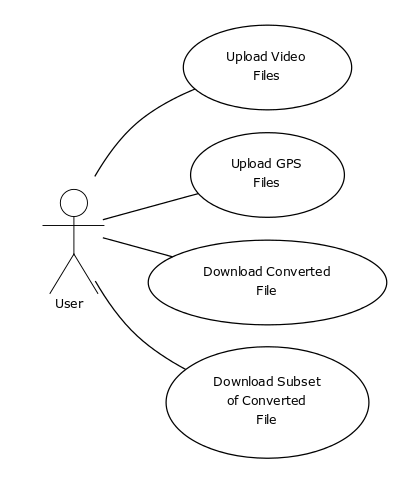
\includegraphics[scale=.4]{images/UCD.png}
\vspace{5mm}

{\Medium\textbf{2.3 Composition Viewpoint}}\\
\vspace{5mm}
The system will be composed of 5 different processes. These include parsing the BLOB files, stabilizing the videos, cropping the videos, correlating the frames of the two videos, and the conversion of the two video files into one stereoscopic 3D video. \\
\vspace{5mm}
2.3.1 Parsing the BLOB file \\
\vspace{3mm}

The role of this process is to extract GPS timestamp data from the BLOB file provided by the camera, so that we can correlate the frames from the two cameras. We found some parsers online, including a Garmin parser on GitHub called Garmin-connect-export [1]. We are unsure if this parser will work, but if need be, we will use reverse-engineering to parse the BLOB files. \\
\vspace{5mm}
2.3.2 Stabilizing the videos\\
\vspace{3mm}

 The role of this process is to take the two videos as input, and output two stabilized videos. For this process, we found functions in the OpenCV library that we will utilize [2]. \\

 \vspace{5mm}
2.3.3 Cropping the videos\\
\vspace{3mm}

The role of this process is to crop the videos so that both videos have equal field of vision. After the stabilization process, there will be black lines on the top and bottom of the videos, so those have to be cropped on both videos so that they will line up when converted to a stereoscopic 3D video. We chose to use functions from OpenCV for this process because they have the necessary tools [3]. \\
\vspace{5mm}

2.3.4 Correlating the frames of the two videos\\
\vspace{3mm}

The purpose of this process is to correlate the frames of the videos using the GPS time stamp data from the BLOB files. This will make it possible to convert the videos into one stereoscopic 3D video.
 \\
 \vspace{5mm}
\newpage
2.3.5 Converting two videos into one stereoscopic 3D video\\
\vspace{3mm}

The purpose of this process is to output the final video in the correct format to view a stereoscopic video in a VR headset. The software we chose to do this process is OpenCV [4].
 \\
\vspace{5mm}

{\Medium\textbf{2.4 Dependency Viewpoint}}\\
\vspace{5mm}

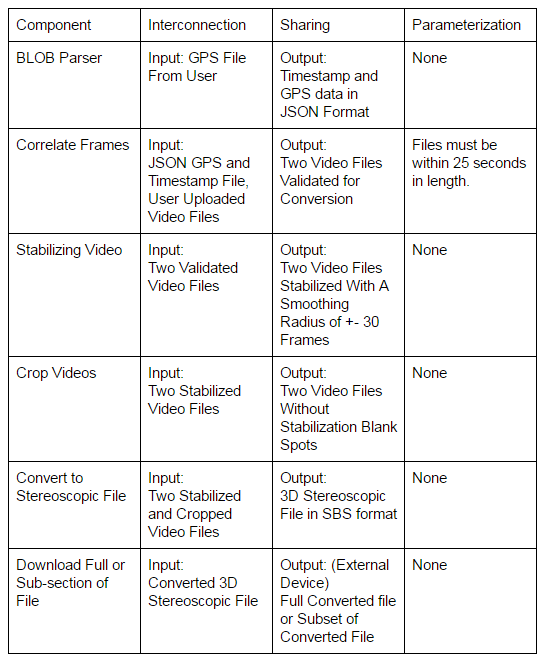
\includegraphics[scale=.8]{images/dependencyDiagram.PNG}\\
Dependency of processes on other processes. \\
\vspace{5mm}
{\Medium\textbf{2.5 Patterns use Viewpoint}}\\
\vspace{5mm}

We will be utilizing the MVC software design pattern for the applications. \\
\vspace{7cm}
{\Medium\textbf{2.6 Interface
Viewpoint}}\\
\vspace{5mm}

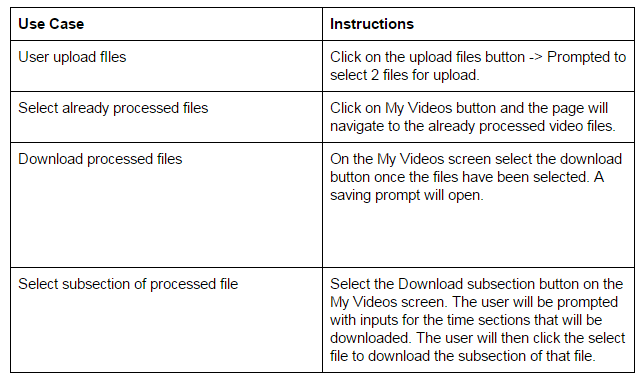
\includegraphics[scale=.8]{images/interface.PNG}\\
\vspace{5mm}
\textbf{2.6.1 Process1: User selects video files to be processed:}\\
\vspace{5mm}
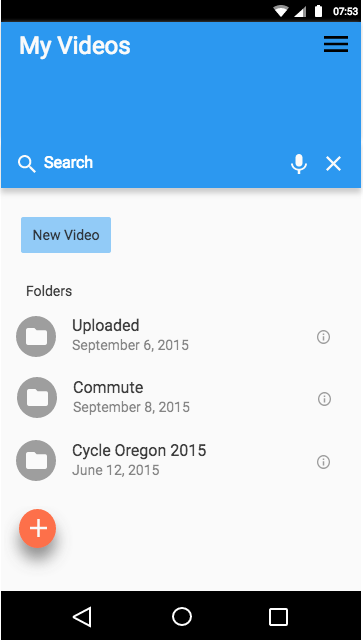
\includegraphics[scale=.47]{images/img1.png}\\
2.6.1.1 User is at My Videos page [7]

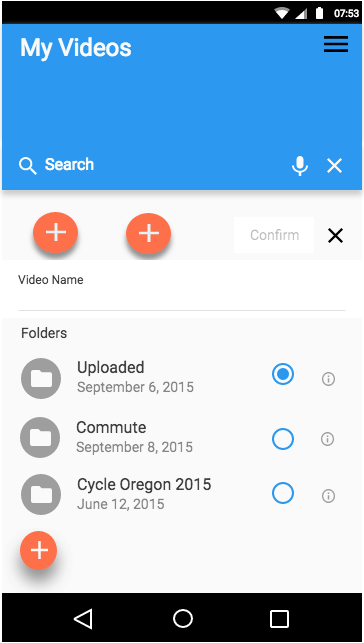
\includegraphics[scale=.47]{images/img2.png}\\
2.6.1.2 User clicks New Video button [7]\\
\vspace{5mm}
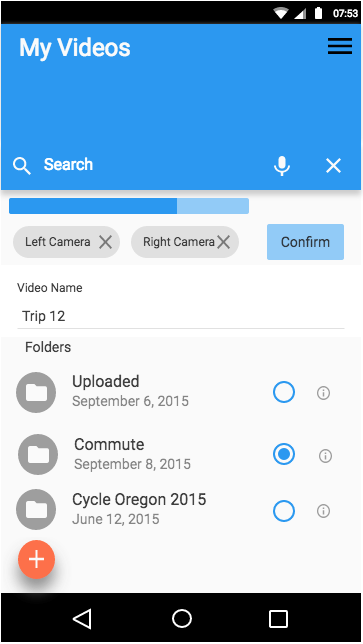
\includegraphics[scale=.47]{images/img3.png}\\
2.6.1.3 User provides two videos stored on devices file system, gives the video a name, and clicks the Confirm button [7]\\
\vspace{5mm}
\newpage
\textbf{2.6.2 Process2: User selects portion of video files to process:}\\
\vspace{5mm}
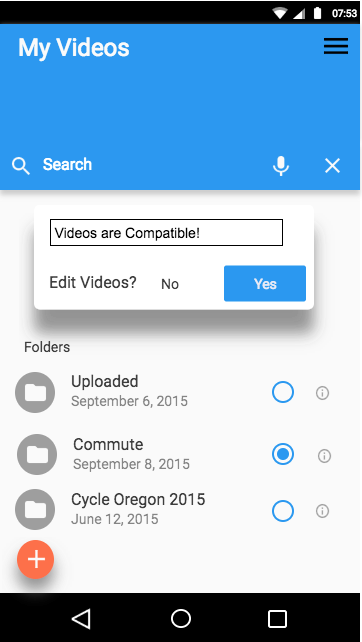
\includegraphics[scale=.47]{images/img4.png}\\
2.6.2.1 User clicks Yes to edit video [7]\\
\vspace{5mm}
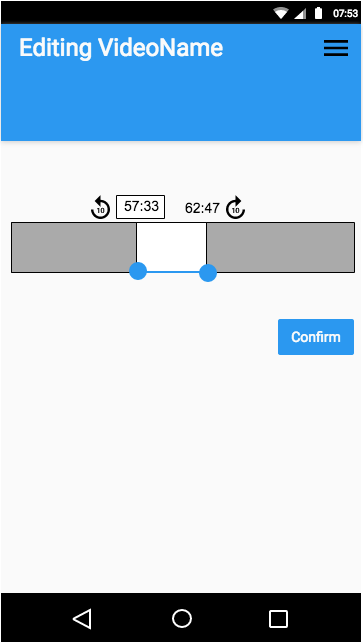
\includegraphics[scale=.47]{images/img5.png}\\
2.6.2.2 Users makes use of video resizing tools to pick a subsection of video to process [7]\\
\vspace{5mm}
\textbf{2.6.3 Process3: Select already processed files:}\\
\vspace{5mm}

2.6.3.1 User is at My Videos page: See 2.6.1.1\\
\vspace{5mm}
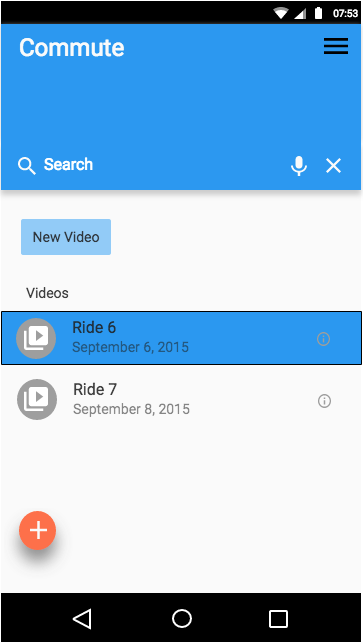
\includegraphics[scale=.47]{images/img6.png}\\
2.6.3.2 User navigates to Commute folder and selects desired video [7]\\
\vspace{5mm}
\newpage
\textbf{2.6.4 Process4: Export processed file:}\\
\vspace{5mm}

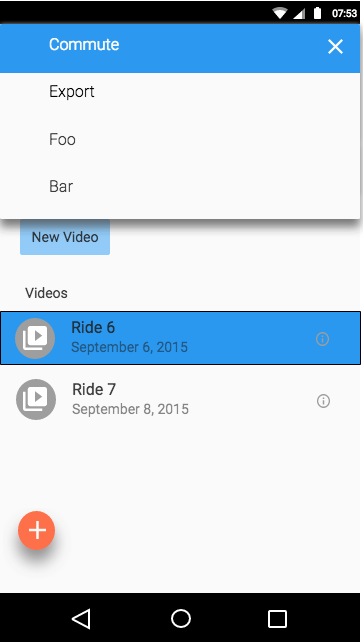
\includegraphics[scale=.47]{images/img7.png}\\
2.6.4.1 User clicks menu expansion button and clicks Export option [7]\\
\vspace{5mm}
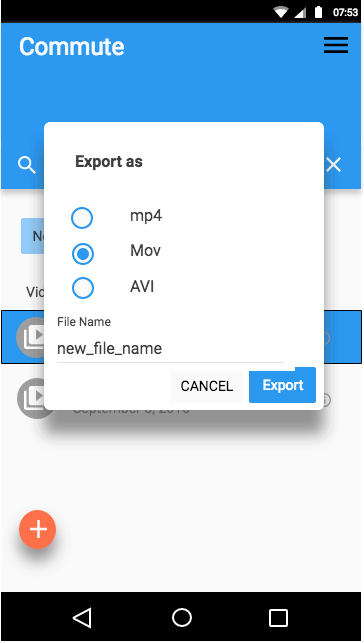
\includegraphics[scale=.47]{images/img8.png}\\
2.6.4.1 User chooses file format to export as and clicks Export button [7]\\
\vspace{5mm}
\textbf{2.6.5 Process4: Select subsection of processed file:}\\
\vspace{5mm}
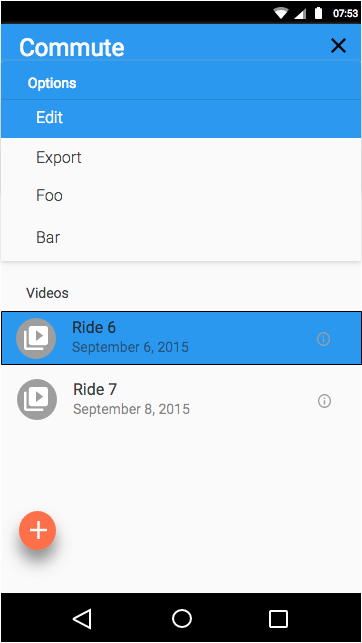
\includegraphics[scale=.47]{images/img9.png}\\
2.6.5.2 Users makes use of video resizing tools to pick a subsection of video to process [7]\\
\vspace{5mm}

2.6.5.1 User clicks menu expansion button and clicks Edit option: See 2.6.2.2\\
\vspace{5mm}

{\Medium\textbf{2.7 Structure Viewpoint}}\\
\vspace{5mm}
UML Class Diagrams for the different processes:\\
\vspace{5mm}
2.7.1 File Upload\\
\vspace{3mm}
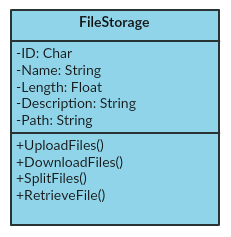
\includegraphics[scale=.8]{images/FileManipClassDiagram.png}\\
\vspace{5mm}
\newpage
2.7.2 Converting Videos\\
\vspace{3mm}
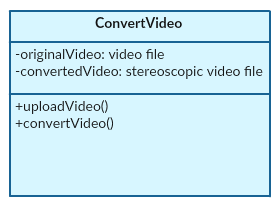
\includegraphics[scale=.8]{images/convertVideo.png}\\
\vspace{5mm}
2.7.3 Parse BLOB\\
\vspace{3mm}
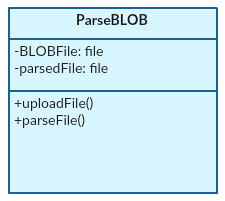
\includegraphics[scale=.8]{images/BLOB.png}\\
\vspace{5mm}
2.7.4 Correlate Frames\\
\vspace{3mm}
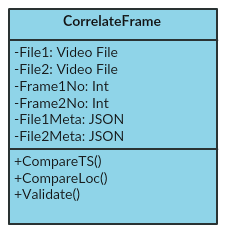
\includegraphics[scale=.8]{images/CorralateFrameDiagram.png}\\
\vspace{5mm}
2.7.5 Crop Videos\\
\vspace{3mm}
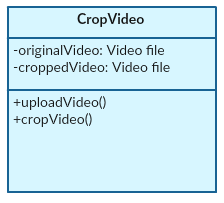
\includegraphics[scale=.8]{images/crop.png}\\
\vspace{5mm}
\newpage
{\Medium\textbf{2.8 Interaction Viewpoint}}\\
\vspace{5mm}
These are how the components of the system will be related and interact with each other. \\
\vspace{5mm}
2.8.1 Relationship 1: The output of the cameras is input for parsing the BLOB files and video stabilization.\\
\vspace{3mm}
2.8.2 Relationship 2: The output of video stabilization will be the input for cropping the videos.\\
\vspace{3mm}
2.8.3 Relationship 3: The output of cropping the videos and output of parsing the BLOB files will be input for correlating frames.\\
\vspace{3mm}
2.8.4 Relationship 4: The output of correlating frames will be input for converting the two videos into one stereoscopic video.\\
\vspace{3mm}
2.8.5 Relationship 5: The output of converting the videos will be input for viewing the 3D video in a VR headset. \\
\vspace{5mm}

{\Medium\textbf{2.9 State Dynamics Viewpoint}}\\
\vspace{5mm}
A State Diagram depicting the flow of data through our system: [6]\\
\vspace{5mm}
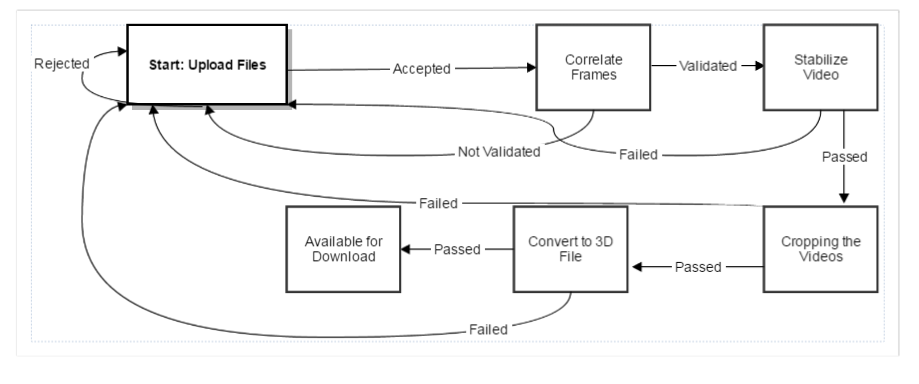
\includegraphics[scale=.7]{images/statediagram.PNG}\\
\vspace{5mm}

{\Medium\textbf{2.10 Algorithm Viewpoint}}\\
\vspace{5mm}
\textbf{2.10.1 Parsing the BLOB file:}\\
\vspace{5mm}
1. This entity will make use of the metadata uploaded by a user of the system. If it is in a recognized format it will apply a known decoding algorithm and reformat the data to a specific format which will be used by the rest of the system.\\
\vspace{3mm}
2. The goal of this process is to reformat the metadata provided by the uploaded video, into a format that can be easily read by the rest of the program.
\vspace{5mm}

\textbf{2.10.2 Stabilizing the videos:}\\
\vspace{5mm}
1. This entity will most likely make use of a third party library to perform the video stabilization process. Our software will provide configuration data to this library. The configuration data will be based off set constants and the video file being processed. \\
\vspace{3mm}
2. The goal of this process is to reduce any shakiness in the video in the hope that the final product will be as stable as possible.
\vspace{5mm}

\textbf{2.10.3 Cropping the videos:}\\
\vspace{5mm}
1. This entity will most likely make use of a third party library to perform the video cropping. The decision of where and how much to crop the videos will be decided based on output from the video stabilization. \\
\vspace{3mm}
\tab a. OpenCV should provide pixel differences between the stabilized and unstabilized videos for each video \tab file. Using this along with the timestamp and gps metadata we can find the largest non-outlier difference \tab between the two files and crop the video at that point.\\
\vspace{3mm}
\tab \tab i. Non-outlier: Find the average y pixel shift at each frame in each video, compare to frame in other \tab \tab video file at the same point, log and find average. Largest non-outlier difference will be the frame \tab \tab that is within 2 standard deviations from average. \\

\vspace{3mm}
2. The goal of this process is to remove vertical portions of the video that greatly differ from each other. These differing portions of video can be caused by the two cameras being set up at slightly differing angles or during the stabilization process.
\vspace{5mm}

\textbf{2.10.4 Correlating the frames of the two videos:}\\
\vspace{5mm}
1. The entity responsible for this process will make use of the metadata formatted by the BLOB parser. It will examine the timestamp data from each metadata file and find the first two frames that are nearest each other. \\
\vspace{3mm}
\tab a. Find video file which started latest. Store timestamp of the first frame captured by it, called start. This \tab frame will be the first frame shown in the relevant side of the three dimensional video. \\
\vspace{3mm}
\tab \tab i. E.g. if the right video file starts later than the left, start will be the first frame shown in the right \tab \tab side. \\
\vspace{3mm}
\tab b. Find frame in other video file which starts closest to start.\\
\vspace{3mm}

\tab \tab i. Search metadata file for first frame that has a timestamp later than start, called post. \\
\vspace{3mm}

\tab \tab ii. Find first frame before post, called pre. \\
\vspace{3mm}

\tab \tab iii. Compare difference between start and post and start and pre.\\
\vspace{3mm}

\tab \tab iv. Smallest timestamp difference found will decide which frame to treat as start of second camera.\\


\vspace{3mm}
2. The goal of this process is to remove vertical portions of the video that greatly differ from each other. These differing portions of video can be caused by the two cameras being set up at slightly differing angles or during the stabilization process.\\
\vspace{5mm}
\textbf{2.10.5 Converting two videos into one stereoscopic 3D video:}\\
\vspace{5mm}
1. This entity will most likely make use of a third party library to combine two processed videos into a single video file. \\

\vspace{5mm}

{\Large\textbf{3 Conclusion}}\\
\vspace{5mm}
In this Software Design Document, we described how we are going to be developing our software, and how all of the components and processes work together. The main part of the system will be composed of several processes and the data flows through the system as follows: The user uploads two videos to the application and begins the conversion process. The videos get stabilized and cropped, then the frames are correlated, and then the two videos get converted into the stereoscopic format. The video is then exported so the user can view the video in a VR headset.

\end{document}
